\documentclass[conference]{IEEEtran}
% Include all packages from file.
% Report template for Mälardalen University
% Original template can be found: 
% https://www.overleaf.com/latex/templates/ieee-bare-demo-template-for-conferences/ypypvwjmvtdf
% Template file structure organised by: Emil Persson
% The following packages should follow the IEEE conference guidelines.

%------------------------------------------------------------------------------------------
% Includes and packages
\usepackage{comment}
\usepackage{amsmath,amssymb,amsfonts}

%------------------------------------------------------------------------------------------
% New commands

\newcommand{\Cov}{\mathrm{Cov}}
\DeclareMathOperator{\atantwo}{atan2}

%------------------------------------------------------------------------------------------
% Swedish language package 
\usepackage[utf8]{inputenc}
\usepackage[T1]{fontenc}
\usepackage[swedish,english]{babel}

% Graphics
\usepackage{graphicx, float, subfigure, blindtext}

\newcommand\IEEEhyperrefsetup{
bookmarks=true,bookmarksnumbered=true,%
colorlinks=true,linkcolor={black},citecolor={black},urlcolor={black}%
}

% Preferred hyperref setup, Michael Shell
\usepackage[\IEEEhyperrefsetup, pdftex]{hyperref}

% Maths
\usepackage{mathtools}

% These packages must be at the end
\usepackage[nolist,nohyperlinks]{acronym}
\usepackage{cleveref}
\graphicspath{{images/}}
%------------------------------------------------------------------------------------------
% Include acronyms
% \acrodef{acronym}[short name]{full name}
\acrodef{IC}[IC]{Integrated Circuit}
% \acrodef{svm}[SVM]{Support Vector Machine}
\newacro{svm}[SVM]{Support Vector Machine}
% Example use \ac{IC} for printing "Integrated Circuit (IC), use \ac{IC} again and it will print (IC)"
% For plural use \acp{IC} for short and \aclp{IC} for long.
% For more see: http://ftp.acc.umu.se/mirror/CTAN/macros/latex/contrib/acronym/acronym.pdf
% Include authors 
\author{\IEEEauthorblockN{
Carl Larsson\IEEEauthorrefmark{1},
Pontus Svensson\IEEEauthorrefmark{2},
}

\IEEEauthorblockA{
School of Innovation, Design and Engineering, M.Sc.Eng Robotics\\
Mälardalens University, Västerås, Sweden\\
Email:
cln20001@student.mdu.se\IEEEauthorrefmark{1}, psn19003@student.mdu.se\IEEEauthorrefmark{2}}
} 
% The report title.
\title{ELA408 - Lab 2\\
Mälardalen University - M.Sc.Eng Robotics Reports}
% Document begins here
\begin{document}
% Create the title.
\maketitle

%------------------------------------------------------------------------------------------
% Example sections, name them
% according to specific needs.
%\begin{abstract}
%------------------------------------------------------------------------------------------

%------------------------------------------------------------------------------------------
\end{abstract}
%\begin{IEEEkeywords}

\end{IEEEkeywords}
\section{Introduction}
%------------------------------------------------------------------------------------------
% Outline

This paper covers lab 2 and consists of the development of an extended Kalman filter (EKF) and particle filter (also known as Sequential Monte-Carlo method) for pose estimation in a landmark map. 
Only the simplest form of matrices are presented here, most matrices can easily be expanded to include e.g. multiple landmarks.
All code developed can be found on \href{https://github.com/MobileLabs408/task_2}{Github}\footnote{https://github.com/MobileLabs408/task\_2} and is open source according to the MIT License.

Hat ($\hat{x}$) is used to denote estimates, $\mathbf{x} = [x,y,\theta]^T$ is used to denote the state of the robot (configuration) and $k$ denotes discrete time steps. Raised to plus sign $x^+$ denotes a prediction from the prediction update and lack of raised plus sign denotes corrected value from correction update.

%------------------------------------------------------------------------------------------
% EKF

\subsection{Extended Kalman Filter}

% Prediction
The EKF prediction update of the state for a differential drive robot can be seen in\:\eqref{eq:prediction_update_state}, and\:\eqref{eq:prediction_update_covariance} presents the covariance matrix of the state uncertainty\:\cite{corke_robotics_2023}.
\begin{equation}
    \begin{split}
        \label{eq:prediction_update_state}
        \hat{\mathbf{x}}^+(k+1) = \mathbf{f}(\hat{\mathbf{x}} (k), \hat{\mathbf{u}} (k),\mathbf{v} (k)) = \\
        =
        \begin{bmatrix}
            x(k) \\
            y(k) \\
            \theta (k)
        \end{bmatrix}
        +
        \begin{bmatrix}
            \delta_d \cos{(\theta (k))} \\
            \delta_d \sin{(\theta (k))} \\
            \delta_{\theta}
        \end{bmatrix}
        +
        \begin{bmatrix}
            v_d \cos{(\theta (k))} \\
            v_d \sin{(\theta (k))} \\
            v_{\theta}
        \end{bmatrix}
        = \\
        =
        \begin{bmatrix}
            x(k) + (\frac{\Delta s_r + \Delta s_l}{2} + v_d) \cos{(\theta (k))} \\
            y(k) + (\frac{\Delta s_r + \Delta s_l}{2} + v_d) \sin{(\theta (k))} \\
            \theta (k) + \frac{\Delta s_r - \Delta s_l}{l} + v_{\theta}
        \end{bmatrix}
    \end{split}
\end{equation}
With control input $\hat{\mathbf{u}} (k) = \mathbf{\delta} (k) = [\delta_d, \delta_{\theta}]^T$ where $\delta_d = \frac{\Delta s_r + \Delta s_l}{2}$ and $\delta_{\theta} = \frac{\Delta s_r - \Delta s_l}{l}$, and $\mathbf{\delta} (k)$ is the odometry measurements\:\cite{corke_robotics_2023}. $l$ is the distance between wheels.
$\mathbf{v} = [v_d,v_{\theta}]^T \sim \mathcal{N}(0, \mathbf{V})$ is the odometry noise, with covariance matrix $\mathbf{V}$ according to\:\eqref{eq:noise_variance}\:\cite{corke_robotics_2023}.
\begin{equation}
    \label{eq:noise_variance}
    \mathbf{V} =
    \begin{bmatrix}
        \sigma_d^2 & 0 \\
        0 & \sigma_{\theta}^2
    \end{bmatrix}
\end{equation}


\begin{equation}
    \label{eq:prediction_update_covariance}
    \hat{\mathbf{P}}^+(k+1) = \mathbf{F}_x \hat{\mathbf{P}}(k) \mathbf{F}_x^T + \mathbf{F}_v \hat{\mathbf{V}} \mathbf{F}_v^T
\end{equation}
Where $\mathbf{F}_x$ is obtained by\:\eqref{eq:f_x} and $\mathbf{F}_v$ by\:\eqref{eq:f_v}\:\cite{corke_robotics_2023}.
\begin{equation}
    \label{eq:f_x}
    \begin{split}
        \mathbf{F}_x = \frac{\partial \mathbf{f}}{\partial \mathbf{x}} \bigg\rvert_{\mathbf{v} = 0} =
        \begin{bmatrix}
            1 & 0 & -\delta_d \sin{(\theta (k))} \\
            0 & 1 & \delta_d \cos{(\theta (k))} \\
            0 & 0 & 1
        \end{bmatrix}
        = \\
        =
        \begin{bmatrix}
            1 & 0 & -\frac{\Delta s_r + \Delta s_l}{2} \sin{(\theta (k))}\\ 
            0 & 1 & \frac{\Delta s_r + \Delta s_l}{2} \cos{(\theta (k))}\\
            0 & 0 & 1
        \end{bmatrix}
    \end{split}
\end{equation}
\begin{equation}
    \label{eq:f_v}
    \mathbf{F}_v = \frac{\partial \mathbf{f}}{\partial \mathbf{v}} \bigg\rvert_{\mathbf{v} = 0} = 
    \begin{bmatrix}
        \cos{(\theta (k))} & 0 \\
        \sin{(\theta (k))} & 0 \\
        0 & 1
    \end{bmatrix}
\end{equation}

%==========================================================================================

% Correction
The EKF correction update of the state for a differential drive robot can be seen in\:\eqref{eq:correction_update_state}, and\:\eqref{eq:correction_update_covariance} presents the covariance matrix of the uncertainty of the state estimate\:\cite{corke_robotics_2023}.
\begin{equation}
    \label{eq:correction_update_state}
    \hat{\mathbf{x}}(k+1) = \hat{\mathbf{x}}^+(k+1) + \mathbf{K} \mathbf{\nu}
\end{equation}
Where $\mathbf{\nu}$ (innovation) is obtained by\:\eqref{eq:innovation}, and $\mathbf{K}$ (Kalman gain) is obtained by\:\eqref{eq:kalman_gain}\:\cite{corke_robotics_2023}.
\begin{equation}
    \label{eq:innovation}
    \begin{split}
        \mathbf{\nu} = \mathbf{z}_i (k+1) - \mathbf{h} (\hat{\mathbf{x}}^+(k+1), \mathbf{p}_i, \mathbf{\omega} (k+1)) = \\
        = \mathbf{z}_i (k+1) -
        \begin{bmatrix}
            \sqrt{(y_i - y_v)^2 ´+ (x_i - x_v)^2} \\
            \atantwo(\frac{y_i-y_v}{x_i-x_v}) - \theta_v
        \end{bmatrix}
        +
        \begin{bmatrix}
            \omega_r \\
            \omega_{\beta}
        \end{bmatrix}
        = \\
        = \mathbf{z}_i (k+1) - 
        \begin{bmatrix}
            \sqrt{(y_i - y_v)^2 ´+ (x_i - x_v)^2} + \omega_r \\
            \atantwo(\frac{y_i-y_v}{x_i-x_v}) - \theta_v + \omega_{\beta}
        \end{bmatrix}
    \end{split}
\end{equation}
Where $\hat{\mathbf{x}}^+(k+1) = [x_v, y_v, \theta_v]^T$ is the predicted estimate state and $\mathbf{p}_i = [x_i, y_i]^T$ is the position of landmark $i$\:\cite{corke_robotics_2023}.
$\mathbf{z}_i (k+1) = [r, \beta]^T$ is the sensor data containing distance and angle to landmark $i$ and $\mathbf{\omega} (k+1) = [\omega_r, \omega_{\beta}]^T \sim \mathcal{N}(0, \mathbf{W})$ is the sensor noise with covariance matrix $\mathbf{W}$ according to\:\eqref{eq:sensor_covariance}\:\cite{corke_robotics_2023}.
%Note that $$\mathbf{h} (\hat{\mathbf{x}}^+(k+1), \mathbf{p}_i) = \begin{bmatrix} \sqrt{(y_i - y_v)^2 ´+ (x_i - x_v)^2} + \omega_r \\ \atantwo(\frac{y_i-y_v}{x_i-x_v}) - \theta_v + \omega_{\beta} \end{bmatrix}$$
\begin{equation}
    \label{eq:sensor_covariance}
    \mathbf{W} = 
    \begin{bmatrix}
        \sigma_r^2 & 0 \\
        0 & \sigma_{\beta}^2
    \end{bmatrix}
\end{equation}
\begin{equation}
    \label{eq:kalman_gain}
    \mathbf{K} = \hat{\mathbf{P}}^+(k+1) \mathbf{H}_x^T (\mathbf{H}_x \hat{\mathbf{P}}^+(k+1) \mathbf{H}_x^T + \mathbf{H}_{\omega} \hat{\mathbf{W}} \mathbf{H}_{\omega}^T)^{-1}
\end{equation}
Where $\mathbf{H}_x$ and $\mathbf{H}_{\omega}$ can be obtained from\:\eqref{eq:h_x} and\:\eqref{eq:h_omega} respectively\:\cite{corke_robotics_2023}.
\begin{equation}
    \label{eq:h_x}
    \mathbf{H}_x = \frac{\partial \mathbf{h}}{\partial \mathbf{x}} \bigg\rvert_{\mathbf{\omega} = 0} =
    \begin{bmatrix}
        -\frac{x_i-x_v}{r} & -\frac{y_i-y_v}{r} & 0 \\
        \frac{y_i-y_v}{r^2} & -\frac{x_i-x_v}{r^2} & -1
    \end{bmatrix}
\end{equation}
Where $r = \sqrt{(y_i - y_v)^2 ´+ (x_i - x_v)^2}$.
\begin{equation}
    \label{eq:h_omega}
    \mathbf{H}_{\omega} = \frac{\partial \mathbf{h}}{\partial \mathbf{\omega}} \bigg\rvert_{\mathbf{\omega} = 0} =
    \begin{bmatrix}
        1 & 0 \\
        0 & 1
    \end{bmatrix}
\end{equation}
\begin{equation}
    \label{eq:correction_update_covariance}
    \hat{\mathbf{P}}(k+1) = \hat{\mathbf{P}}^+(k+1) - \mathbf{K} \mathbf{H}_x \hat{\mathbf{P}}^+(k+1)
\end{equation}

%------------------------------------------------------------------------------------------
% Particle Filter

\subsection{Particle Filter}
% Prediction
Particle filter starts by initializing $N$ number of state samples (particles) in a random uniform distribution. Initially all particles have weight $w_i = 1/N$\:\cite{corke_robotics_2023}.
The particle filter prediction update of the state for a differential drive robot can be seen in\:\eqref{eq:pf_state_update}, and is applied to each particle $i$\:\cite{corke_robotics_2023}.
\begin{equation}
    \label{eq:pf_state_update}
    \begin{split}
        \mathbf{x}_i^+(k+1) = \mathbf{f}(\mathbf{x}^+_i(k), \hat{\mathbf{u}}(k), \mathbf{r}(k)) = \\
        =
        \begin{bmatrix}
            x(k) \\
            y(k) \\
            \theta (k)
        \end{bmatrix}
        +
        \begin{bmatrix}
            \delta_d \cos{\theta(k)} \\
            \delta_d \sin{\theta(k)} \\
            \delta_{\theta}
        \end{bmatrix}
        +
        \begin{bmatrix}
            r_d \cos{\theta(k)} \\
            r_d \sin{\theta(k)} \\
            r_{\theta}
        \end{bmatrix}
        = \\
        =
        \begin{bmatrix}
            x(k) + (\frac{\Delta s_r + \Delta s_l}{2} + r_d) \cos{(\theta (k))} \\
            y(k) + (\frac{\Delta s_r + \Delta s_l}{2} + r_d) \sin{(\theta (k))} \\
            \theta (k) + \frac{\Delta s_r - \Delta s_l}{l} + r_{\theta}
        \end{bmatrix}
    \end{split}
\end{equation}
Where $\hat{\mathbf{u}}(k)$ is the control input, which is equal to the measured odometry $\hat{\mathbf{u}} (k) = \mathbf{\delta} (k) = [\delta_d, \delta_{\theta}]^T$\:\cite{corke_robotics_2023}, with $\delta_d = \frac{\Delta s_r + \Delta s_l}{2}$ and $\delta_{\theta} = \frac{\Delta s_r - \Delta s_l}{l}$. With random variables $r_d \sim U(a_d, b_d)$ and $r_{\theta} \sim \text{Logistic}(\mu_{\theta}, s_{\theta})$, $\mathbf{r}(k)$ is used to spread out all the particles\:\cite{corke_robotics_2023}. $l$ is the distance between the wheels.

% Update
Then follows the update phase, where first the innovation for each particle $i$ to landmark $j$ is calculated according to\:\eqref{eq:pf_nu}\:\cite{corke_robotics_2023}.
\begin{equation}
    \label{eq:pf_nu}
    \begin{split}
        \mathbf{\nu}_i = \mathbf{h} (\mathbf{x}_i^+(k+1), \mathbf{p}_j, \mathbf{\omega} (k+1)) - \mathbf{z}_j (k+1) = \\
        = 
        \begin{bmatrix}
            \sqrt{(y_j - y_v)^2 ´+ (x_j - x_v)^2}\\
            \atantwo(\frac{y_j-y_v}{x_j-x_v}) - \theta_v
        \end{bmatrix}
        +
        \begin{bmatrix}
            \omega_d \\
            \omega_{\beta}
        \end{bmatrix}
        - \mathbf{z}_j (k+1)
        = \\
        =
        \begin{bmatrix}
            \sqrt{(y_j - y_v)^2 ´+ (x_j - x_v)^2} + \omega_d \\
            \atantwo(\frac{y_j-y_v}{x_j-x_v}) - \theta_v + \omega_{\beta}
        \end{bmatrix}
        - \mathbf{z}_j (k+1)
    \end{split}
\end{equation}
Where $\mathbf{p}_j = [x_j, y_j]^T$ is the position of landmark $j$, $\mathbf{z}_j$ is the observation of landmark $j$ and $\mathbf{x}_i^+(k+1) = [x_v, y_v, \theta_v]^T$\:\cite{corke_robotics_2023}. With sensor noise $\mathbf{\omega} (k+1)$ which consists of $\omega_d \sim \text{Logistic} (0,s_d)$ and $\omega_{\beta} \sim \text{Logistic} (0, s_{\beta})$.

Then the weights for all particles are updated according to\:\eqref{eq:pf_weight}\:\cite{corke_robotics_2023}.
\begin{equation}
    \label{eq:pf_weight}
    w_i = e^{-\mathbf{\nu}_i^T \mathbf{L}^{-1} \mathbf{\nu}_i} + w_0
\end{equation}
Where $w_0 > 0$ and $\mathbf{L}$ is the covariance matrix according to\:\eqref{eq:L_covariance_matrix}\:\cite{corke_robotics_2023}.
\begin{equation}
    \label{eq:L_covariance_matrix}
    \mathbf{L} = 
    \begin{bmatrix}
        s_d^2 & 0           \\
        0     & s_{\beta}^2
    \end{bmatrix}
\end{equation}
The weights are then normalized according to\:\eqref{eq:pf_weight_update}\:\cite{corke_robotics_2023}.
\begin{equation}
    \label{eq:pf_weight_update}
    w'_i = \frac{w_i}{\sum_{n = 1}^N w_n}
\end{equation}

The estimated position is calculated according to the weighted sum of all particles, see\:\eqref{eq:weighted_sum}.
\begin{equation}
    \label{eq:weighted_sum}
    \hat{\mathbf{x}} (k+1) = \sum_{i=1}^N w'_i \cdot \mathbf{x}_i^+(k+1)
\end{equation}

Lastly, resampling is done by low variance resampling (stochastic universal resampling), which works by forming cumulative histograms (see\:\eqref{eq:cumulative_histograms}\:\cite{corke_robotics_2023}) of all the weights of all particles. Then a random number $r \in [0, \frac{1}{N}]$ is generated, the particle $i$ which $r$ "lands on" and all other particles which $r + n\frac{1}{N}, n = 1,2,...,N$ "lands on" are selected for resampling (be part of the next set), resulting in $N$ samples in the set of particles each iteration.  
\begin{equation}
    \label{eq:cumulative_histograms}
    c_j = \sum_{i = 1}^j w'_i
\end{equation}

%------------------------------------------------------------------------------------------


%------------------------------------------------------------------------------------------
\begin{comment}
    \subsection{Assignment}
    \subsubsection{Theoretical equations for the differential drive robot}
    \begin{itemize}
        \item \textbf{EKF}: prediction
        \item \textbf{EKF}: correction
    \end{itemize}
\end{comment}
%------------------------------------------------------------------------------------------
%\section{Method}
%------------------------------------------------------------------------------------------

%------------------------------------------------------------------------------------------


%------------------------------------------------------------------------------------------
\begin{comment}
    
\end{comment}
%------------------------------------------------------------------------------------------
\section{Results}
%------------------------------------------------------------------------------------------

\subsection{Extended Kalman Filter}
The reconstructed trajectory by EKF can be seen in Fig.\:\ref{fig:EKF_trajectory}, and the components with respect to time can be seen in Fig.\:\ref{fig:EKF_subplot}, both also containing original trajectory for reference.
% Trajectory
\begin{figure}
    \centering
    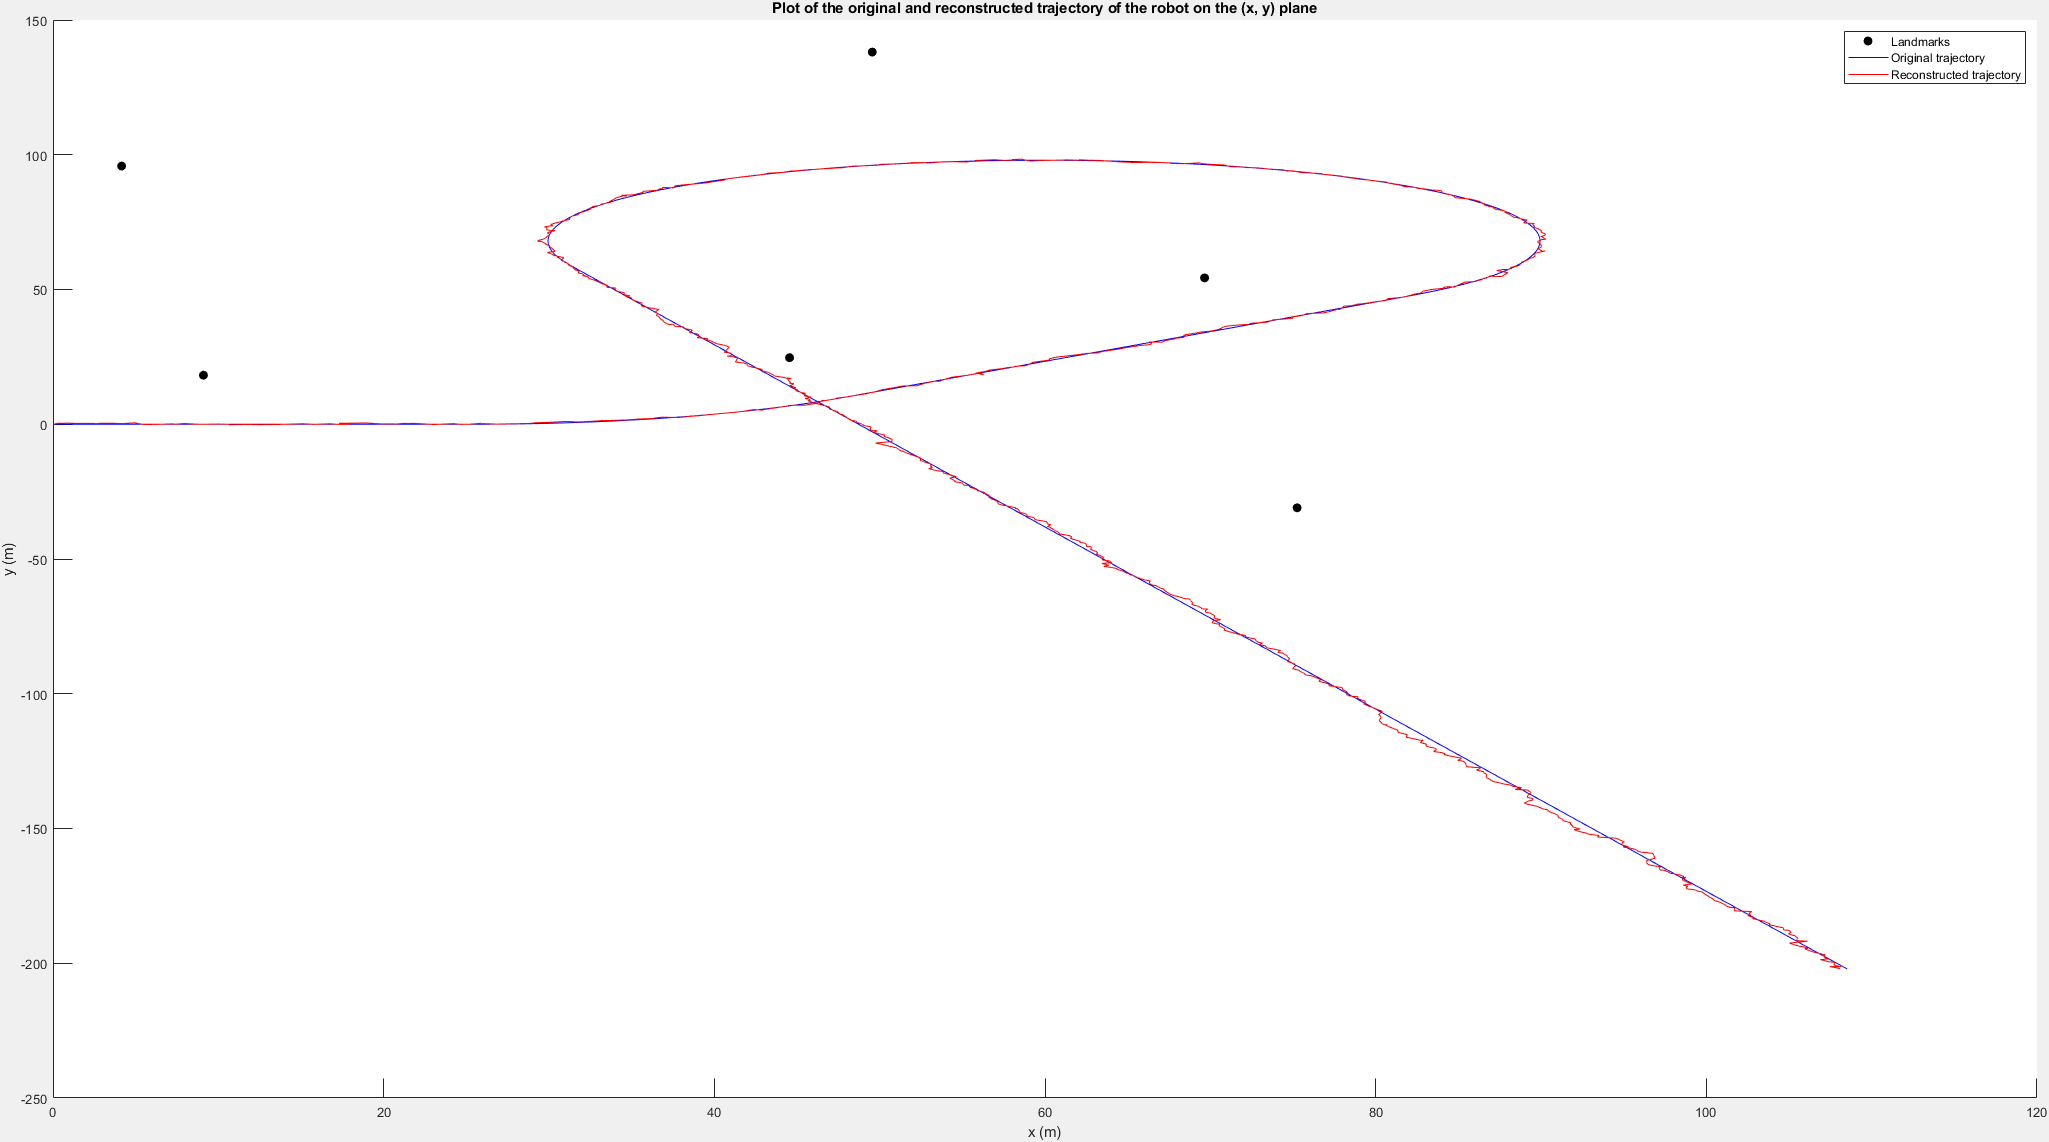
\includegraphics[width=\columnwidth]{images/EKF_trajectory.png}
    \caption{Original and reconstructed trajectory by EKF.}
    \label{fig:EKF_trajectory}
\end{figure}
% Subplots
\begin{figure}
    \centering
    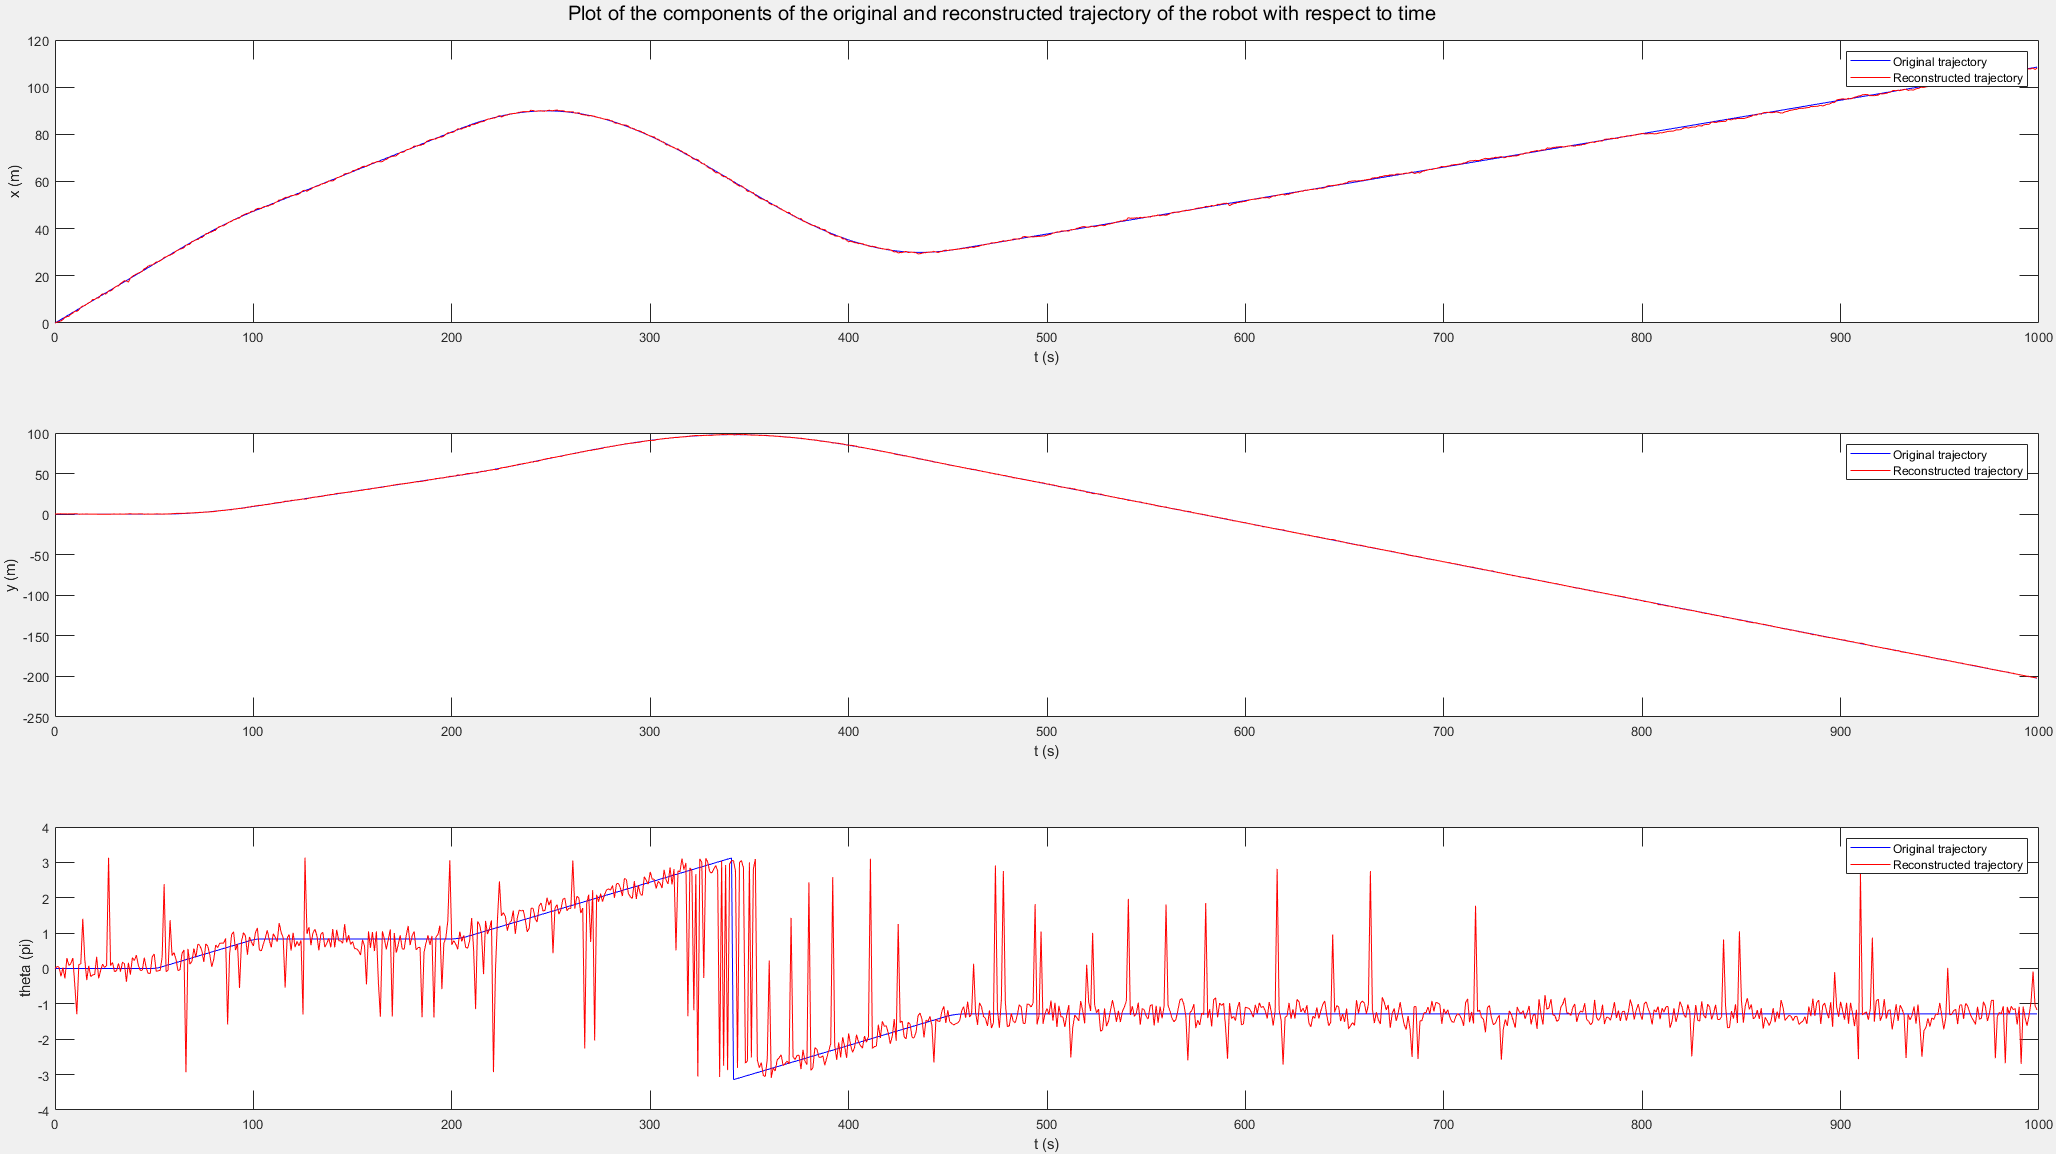
\includegraphics[width=\columnwidth]{images/EKF_subplot.png}
    \caption{Original and reconstructed trajectory components with respect to time by EKF.}
    \label{fig:EKF_subplot}
\end{figure}

%------------------------------------------------------------------------------------------

\subsection{Particle Filter}
The execution time for the particle filter with some example number of particles is shown in Table.\:\ref{tab:execution_time}.
% Compare the results of using 100, 500, 1000 and 3000 particles, report the execution time for each particle set.
\begin{table}
    \centering
    \begin{tabular}{c|c|c|c|c}
        Particles          & $100$      & $500$         & $1000$        & $3000$        \\ 
        \hline
        Execution time (s) & $3.0541$   & $16.2611$     & $31.4827$     & $95.6879$
    \end{tabular}
    \caption{Execution time for particle filter for some example number of particles.}
    \label{tab:execution_time}
\end{table}
Fig.\:\ref{fig:pf_trajectory} shows the trajectory for the particle filter and Fig.\:\ref{fig:pf_subplot} shows the trajectory components as functions of time when using $3000$ particles, both figures containing original trajectory for reference.
% Trajectory
\begin{figure}
    \centering
    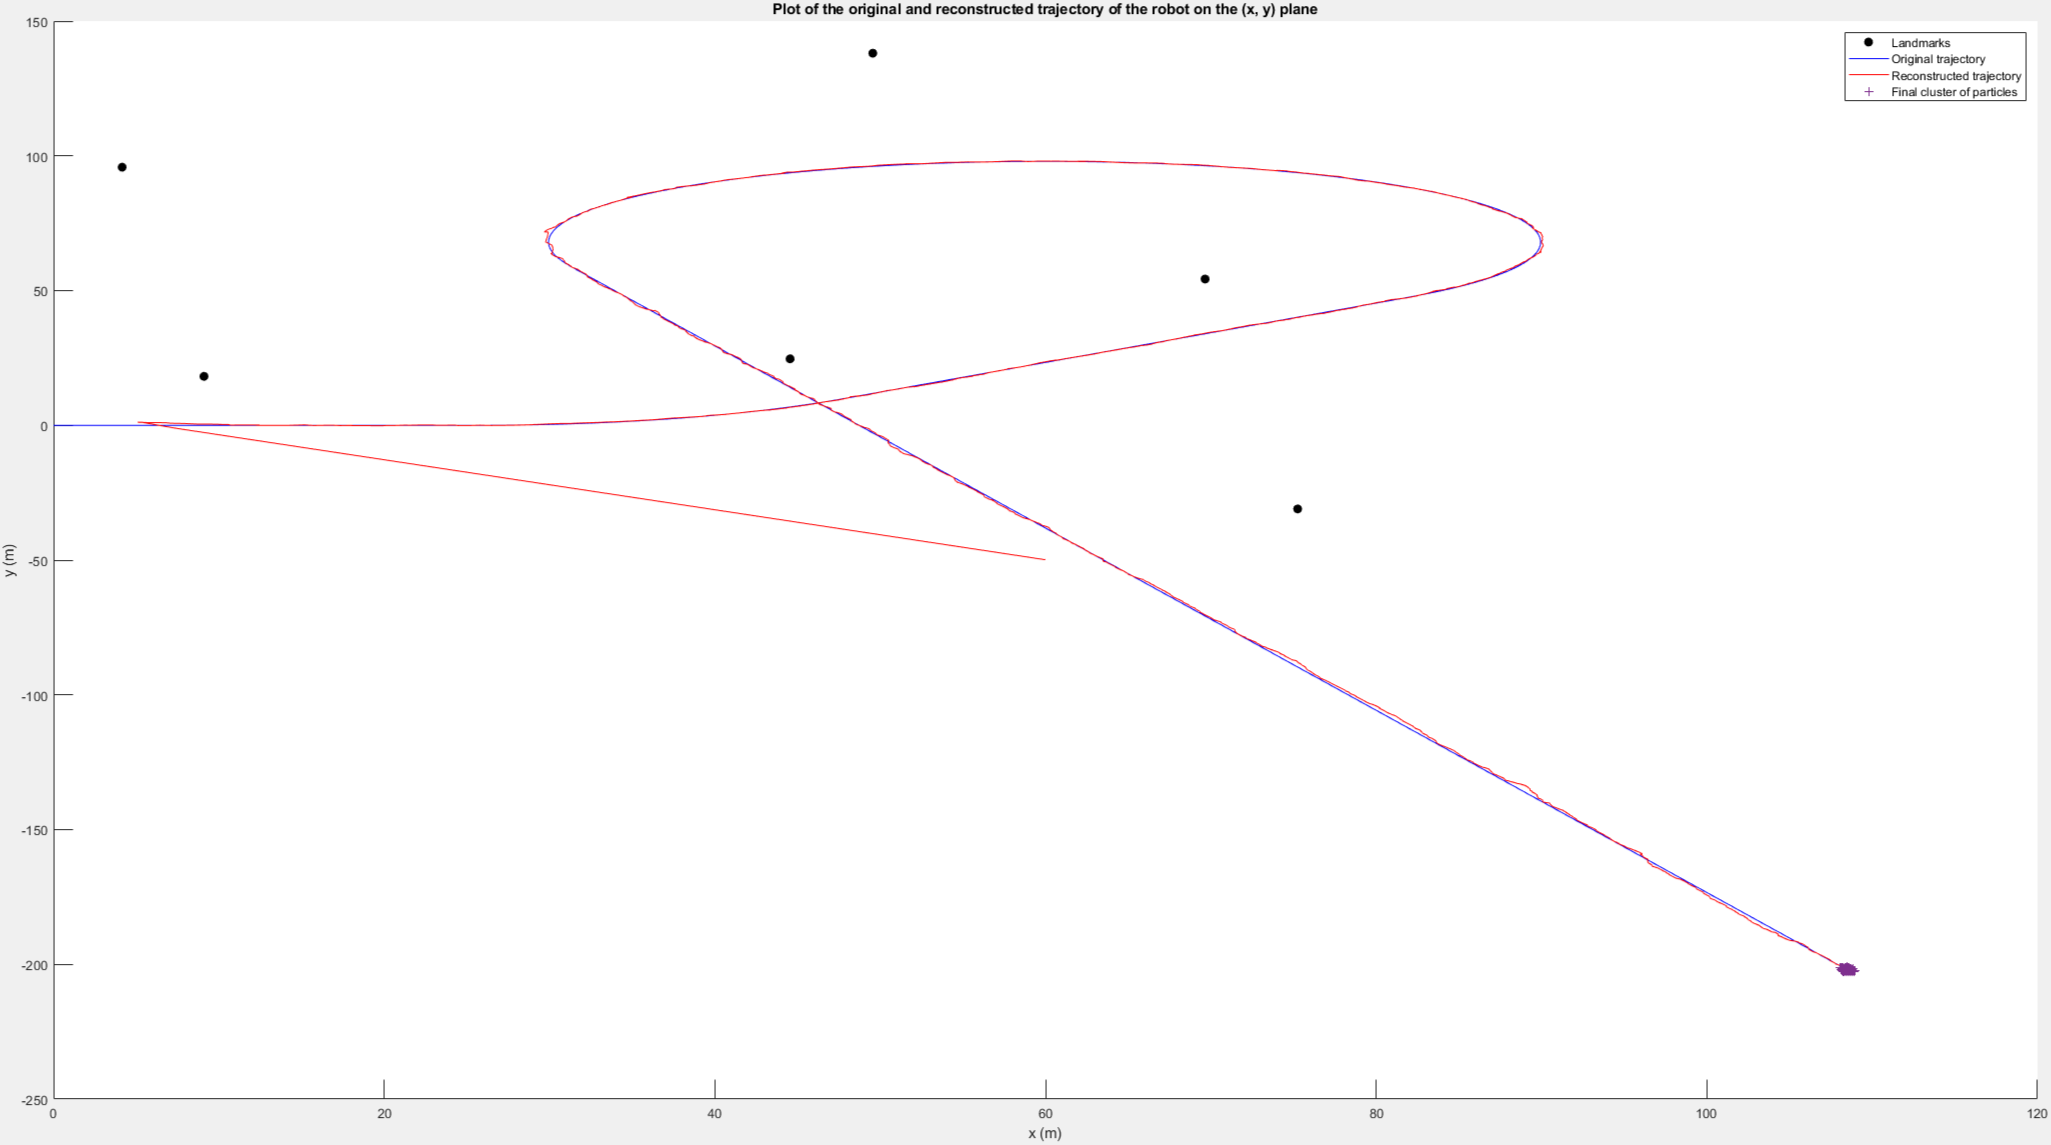
\includegraphics[width=\columnwidth]{images/pf_trajectory.png}
    \caption{Particle filter reconstructed trajectory using 3000 particles and original trajectory.}
    \label{fig:pf_trajectory}
\end{figure}
% Subplots
\begin{figure}
    \centering
    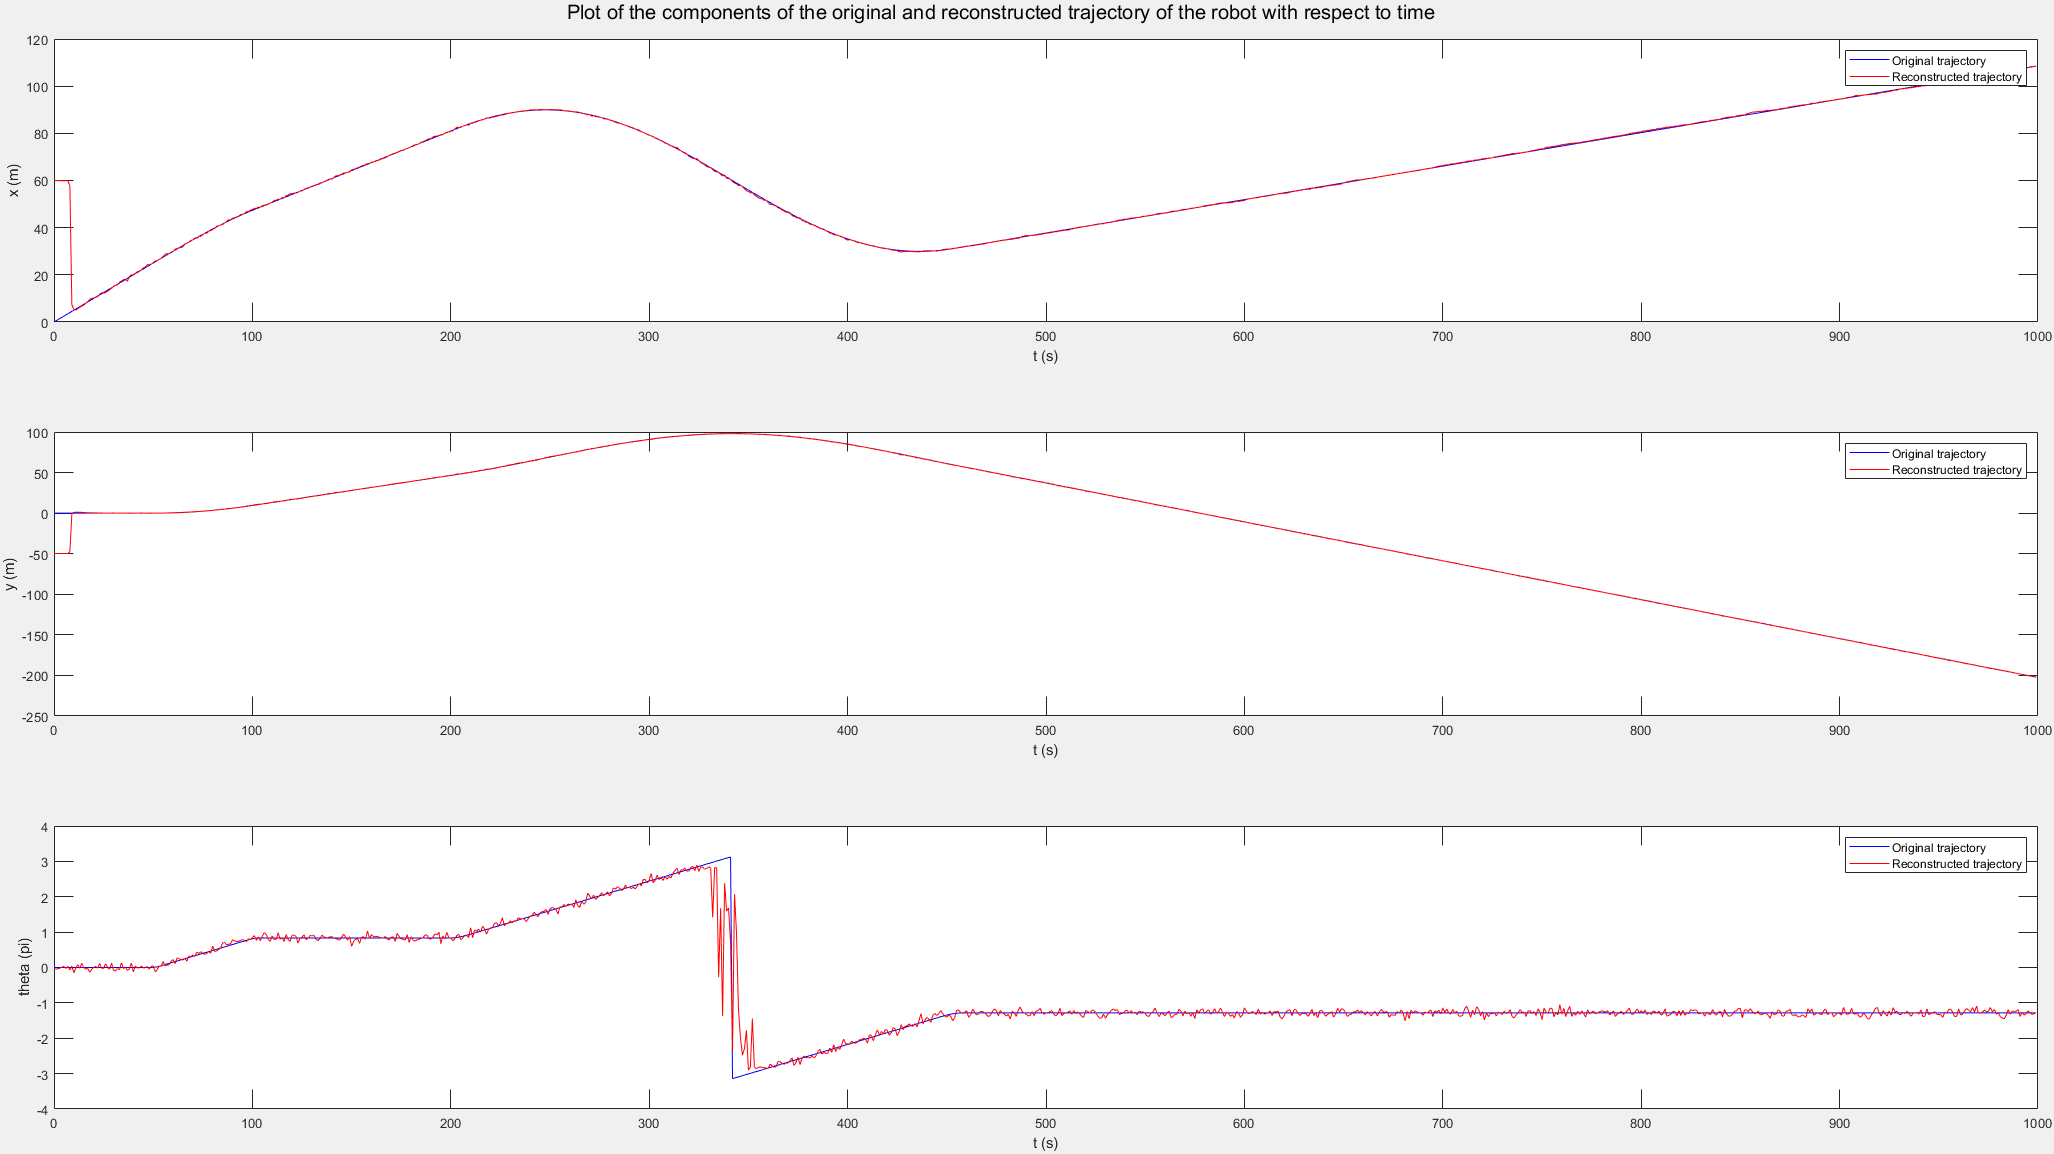
\includegraphics[width=\columnwidth]{images/pf_subplot.png}
    \caption{Particle filter reconstructed trajectory components as a function of time using 3000 particles, with original trajectory for reference.}
    \label{fig:pf_subplot}
\end{figure}

%------------------------------------------------------------------------------------------


%------------------------------------------------------------------------------------------
\begin{comment}
    
\end{comment}
%------------------------------------------------------------------------------------------
%\section{Discussion}
\label{section:disc}

%\section{Conclusion}
%\section*{Acknowledgment}

%------------------------------------------------------------------------------------------
% Select the IEEEtran style
\bibliographystyle{IEEEtran}
% Include bibliography file
\bibliography{refs,ELA408}
%------------------------------------------------------------------------------------------

\end{document}